\chapter{PET Adoption Considerations}

Several factors affect the accuracy of the model and there are several points of
tuning and optimization throughout the workflow. We now consider the steps
needed to adapt the use of PET on a new CPU platform. First, one must create a
CPU model using gem5's Python interface, resembling the modelled hardware. Then,
finding correct weights is formulated as a global optimization problem.


\section{Simulator Environment}

PET relies heavily on a front-end that can execute a binary on a simulator and
output $(time, event)$ tuples as a trace of execution. In this thesis, we are
using the gem5 simulator, but technically PET could be modified to support any
simulator front-end. The power profile generated by PET are derived from the
weight configuration given as input and the simulation trace, so it is important
that the simulator trace is similar to a hardware execution.

Butko et al. \cite{butko2012accuracy} reports gem5 accuracy to vary from 1.39\%
to 17.94\%, with the most accurate results coming from programs with low memory
usage. The benchmarks used represents a wide variety of scientific workloads, as
well as media applications and memory intensive synthetic benchmarks. The
program execution for their benchmarks has a high degree of instruction
diversity, so they get away with having a very simple CPU model. The real
program flow gets diluted and accurate timings are obtained simply by setting
the correct CPI value. In fact, they even use an in-order model to simulate an
out-of-order core.

We claim that the key to obtain high precision power estimates is an
architectural simulator with great accuracy. The simulator must exhibit similar
timing characteristics as the target hardware under all workloads considered,
such that the simulated execution resembles the hardware execution as much as
possible. The scheme suggested in this thesis is based on accumulation of
discrete events, each with an assigned weight according to its contribution to
the global power consumption. This means that accurate power estimation needs
these discrete events to happen, and they must happen with a realistic timing
related to their triggering cause.

Without a simulator capable of providing decent accuracy over system events,
power estimation using methods as suggested in this report will fail. We will
now explain how gem5 can be configured to improve simulator accuracy for a
particular CPU core, as well as pointing out difficulties with this approach.


\subsection{gem5 CPU configuration}
The gem5 simulator is bundled with an out-of-order ARMv7 core and serves as a
basis for the evolution of our custom core meant to model an A9 core on the
Exynos 4412. ARM cores can be configured with caches of varying sizes decided
by the implementing vendor and will have varying performance accordingly. Thus,
it is important to tune all CPU parameters so that it matches the modelled SoC.
It is not publicly known which SoC the default configuration attempts to model,
but according to the gem5 mailing list \cite{a15maillist} it is neither A9 or
A15. However, the fact that it is made for the ARMv7 instruction set and is
out-of-order makes us believe minor modifications can make it a decent model of
the Cortex-A9.

The model gem5 uses in its simulations can easily be configured using a Python
interface. We started with gem5 changeset \texttt{aaf017eaad7d} and added a new
CPU configuration file for the Exynos 4412;
\texttt{gem5/configs/common/Exynos\_4412P.py}. A few other files were edited to
accomodate the new processor definition. Please refer to
\autoref{apx:gem5files} to see all patches applied in these experiments.

As implementation details for commercial processors are hidden from the end
user, the Internet can deem helpful in the search for clues. We found many
sources of information claiming to know implementation details of the Cortex-A9,
including
\cite{blem2013detailed,butko2012accuracy,armtech,exynoswiki,odroidwiki,geekland,7cpu,armcortexa9specs}.

Combining this information helps us build a gem5 model for the Exynos SoC, but
it is still not trivial.  We found the simulator to perform different from the
physical hardware, even though the system parameters are set equal. We claim
that this is due to the abstraction the simulator provides us; the simulator is
not a complete model of the hardware. Gibson et. al. \cite[gibson2000flash] have
done a similar experiment using different simulators and concluded that bugs and
ommisions in system simulators may make performance tuning very difficult.

To improve our results, we adjust the model specification such that it
\textit{performs} similar to the hardware, i.e.  programs execute in about the
same number of clock cycles. Even if the processor implementation was completely
transparent, it would be hard to leverage the use of a multi-architecture
computer simulators. Features such as fast-loop mode found in certian ARM cores
must have a corresponding implementation in the simulator for complete
correctness, and it would be infeasible to include all details at that
granularity.

We scripted the simulator to run a wide variety of configurations, about $50$ in
total. We evaluated their performance by comparing simulated execution time to
execution time on real hardware. The final CPU configuration is shown in its
entirity in \autoref{gem5exynos4412p}.


\subsection{gem5 memory model}
The memory system is a very important part of a system simulator when doing performance estimations, but
in the time of writing, gem5 will not easily work with an out-of-order CPU model together with the GEMS Ruby
memory system. Lacking other methods considering our resources, the simple memory system will provide events
that PET can use to determin memory and memory bus communications. The simple memory model was tuned as stated
in \autoref{gem5simpledram}.

\section{Multi-objective Weight Optimization}

With an accurate CPU model, the weights must now be tuned to match measured
power consumption on real hardware. We formulate this as a multi-objective
optimization problem.

We start by creating a set of training workloads, essentially computer programs
designed to hold certain characteristics compiled to a native
ARMv7\footnote{ARMv7 is the instruction set supported by ARM Cortex-A9.} binary.
The design and selection of these will be elaborated in the next section. We
execute the binaries in the gem5 simulator with the CPU model from last
section to obtain a file containing \texttt{(time, event)} tuples from the
(modelled) execution, just like in \autoref{lst:trace}. The next challenge is to
assign each of these events a cost.

We attack this problem by running a multi-objective optimization algorithm. We
pick a subset of event types that is believed to impact energy consumption, as
we described in \autoref{subsec:powerevents}.

%TODO: Any kind of opt.alg. could have been used


We tested many evolutionary strategies
and were able to prototype quickly using DEAP \cite{DEAP_JMLR2012}, a Python
framework for evolutionary algorithms. In the end, we do not care how the
weights are found, as long as they match well to the hardware measurements.
Please note that any optimization algorithm could be used to find a proper set
of weights.

The genome is a set of CPU events, each mapped to an energy cost. E.g.
\texttt{\{IntAlu: 170, IntMult: 1300, MemRead: 80, MemWrite: 50, SimdFloatMisc:
1400, L1R: 230, L1W: 340, L2R: 1100, L2W: 1300, PhysR: 2600, PhysW: 2800\}} is a
valid individual in the population. To calculate the fitness of an individual,
we run PET with the genome weights on a set of workloads and compare the energy
profiles with measurements on hardware. Note that hardware measurements only
needs to be done once per workload. The evolution can now run without
supervision until a set of reasonable weights are evaluated.

\section{Choosing Workloads}
\label{sec:workloads}

When running a genetic algorithm, it is critical to lead the evolution in the
correct direction. In our case, this is done by providing a reasonable set of
workloads (i.e. ARMv7 programs) that stresses distinct modules in the processor.
For instance, a memory intensive workload will have high density of
memory-related events from the simulator, and will support the genetic algorithm
in determining cost for memory accesses. It is important for the set of
workloads that are chosen to be diverse and stress many conditions the processor
can operate in, e.g. mixes of compute intensive and memory intensive programs. A
poorly chosen set of workloads will not give a fair judgment on which genomes
that fit well. A bad workload might be too biased towards a few parameters,
neglecting the rest, or even mislead the GA into a local optimum
\cite{introtoga}. All training programs are compiled with soft-floats to keep
simulation complexity low. Another worry is that within the training set, there
will most likely exist multiple Pareto optimal solutions \cite{deb2014multi},
but only one of these can truly match the real power consumption.

We came up with the following four workloads.

\begin{description}
    \item[Pi] \hfill \\
        This test calculates Pi using Monte Carlo simulation. It includes
        floating point multiply and division. It runs for a fixed amount of
        iterations.
    \item[SHA-512] \hfill \\
        The SHA-512 algorithm is a hashing algorithm used in cryptography. It
        includes a mix of integer operations and memory usage. Implementation
        from \cite{sha2}.
    \item[Trend] \hfill \\
        This test has two parts. It starts with a tight add loop, and then
        continues with extensive memory allocation. Presumably, this will create
        a shift in energy consumption between the two stages.
    \item[SubMul] \hfill \\
        The SubMul test borrows ideas from the previous program, but instead of
        testing ALU and memory, this test compares subtract and multiply (both
        ALU).
\end{description}

We claim that the workloads used in this experiment spans the most common
instruction types while being simple enough to be simulated in gem5 on
reasonable time.


\section{Results}

\subsection{gem5 CPU model accuracy}

After modelling different configurations for gem5, accuracy as depicted in \autoref{tbl:gem5runtimeaccuracy}
was achieved. Each test was run with the command written out in \autoref{lst:gem5commandline}, with \texttt{CPU}
changed with  \texttt{exynos\_4412p}, \texttt{arm\_detailed} and \texttt{timing}.

\begin{lstlisting}[language=sh,label={lst:gem5commandline},caption={gem5 Command Line}]
$ build/ARM/gem5.opt --remote-gdb-port=0 -d m5out-time/sha2-sha2
    configs/example/se.py -c bin/sha2/sha2 --cpu-type=CPU
    --mem-type=LPDDR2_S4_800_x32 --sys-clock=440MHz
    --cpu-clock=1700MHz --num-l3caches=0 --caches --l2cache
    --l2_assoc=16 --l2_size=1MB --l1d_size=32kB
    --mem-size=2048MB --l1d_assoc=4 --l1i_assoc=4
\end{lstlisting}


% Move table to result chapter
\begin{table}
\centering
\begin{tabular}{|l|c|c|c|c|}
\hline
 & add-add & pi-pi & sha2-sha2 & trend-trend \\
\hline
Real hardware & 0.017600  & 0.013500 & 0.022600 & 0.014600 \\
gem5 modified O3    & 0.017541 & 0.013790 & 0.022819 & 0.011898 \\
gem5 original O3    & 0.008777 & 0.006708 & 0.010368 & 0.004344 \\
gem5 timing simple  & 0.035039 & 0.019564 & 0.040659 & 0.020503 \\
\hline
\end{tabular}
\caption{gem5 runtime accuracy (O3 with classic memory system)}
\label{tbl:gem5runtimeaccuracy}
\end{table}




\subsection{GA optimization}
As PET has been optimized by a genetic inspired algorithm, it is likly to perform very well on the data sets it
has been optimized for. When such training is done, a controll test is needed in order to verify that the result
is good for the general problem solved, not only the specific instances used for training.

\subsection{Training}

The training sets:
\begin{figure}
\centering
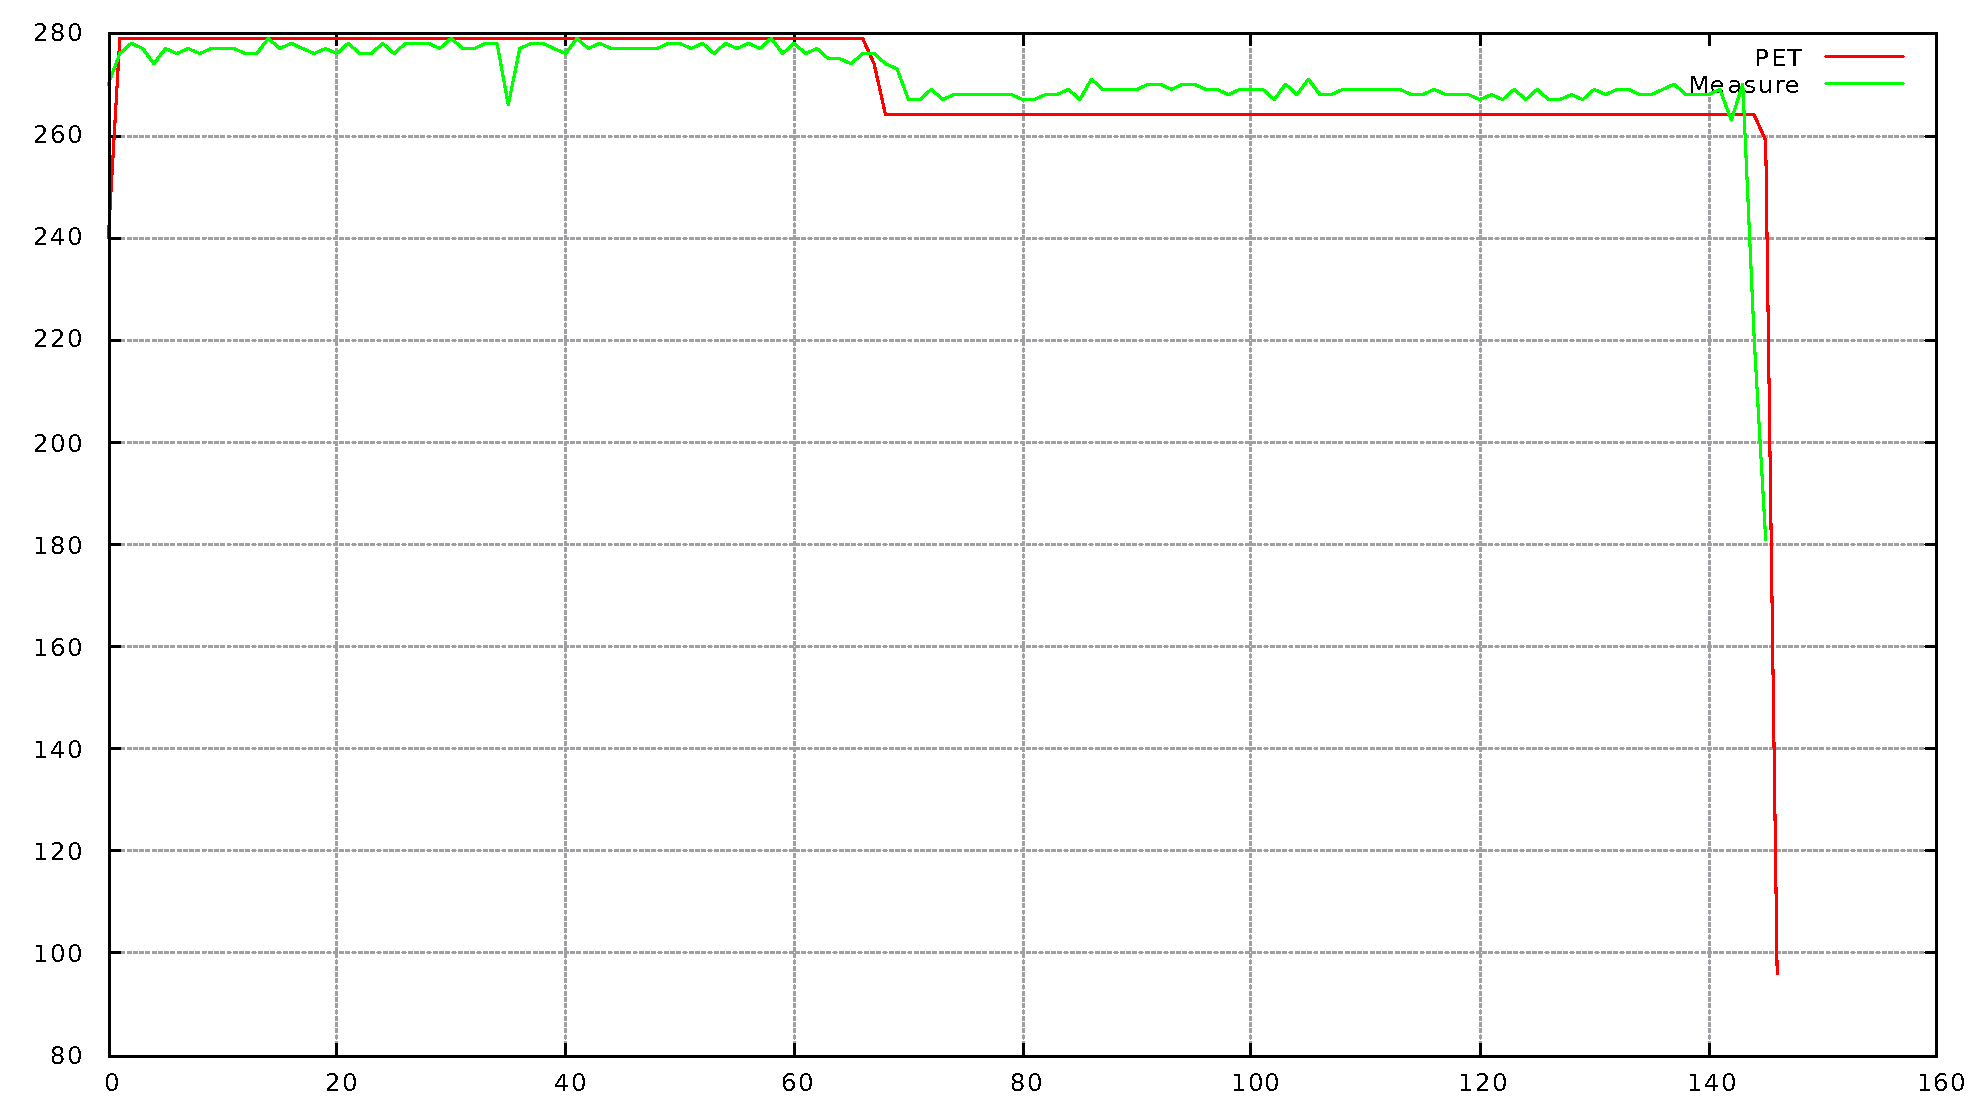
\includegraphics[width=\textwidth]{figs/trend-training.pdf}
\caption{Overlay of PET training results (red) and training data (green)}
\label{fig:trend-training}
\end{figure}



